\documentclass[conference]{IEEEtran}
\IEEEoverridecommandlockouts

\usepackage{cite}
\usepackage{amsmath}
\usepackage{amsthm}
\usepackage{newtxtext,newtxmath}
\usepackage{graphicx}
\usepackage{stfloats}
\usepackage{booktabs}
\usepackage{algorithm}
\usepackage[noend]{algpseudocode}
\usepackage{xcolor}
\usepackage[hidelinks]{hyperref}

\newtheorem{lemma}{Lemma}
\newtheorem{proposition}{Proposition}
\newtheorem{fact}{Fact}
\theoremstyle{definition}
\newtheorem{definition}{Definition}

\newcommand{\W}{W}
\newcommand{\capr}{\mathrm{cap}_\rho}
\newcommand{\BAD}{\mathit{BAD}}
\newcommand{\maj}{\mathit{maj}}
\newcommand{\kw}[1]{\textbf{#1}}
\newcommand{\varind}{\hphantom{\kw{var}}}
\newcommand{\midrulefill}{\leavevmode\leaders\hrule height \dimexpr.5ex+.2pt\relax depth -\dimexpr.5ex-.2pt\relax\hfill\kern0pt}
\newcommand{\sep}[1]{\ifx\relax#1\relax\hrulefill\else\midrulefill\enspace\textit{#1}\enspace\midrulefill\fi}
\newcommand{\ind}{\hspace*{\algorithmicindent}}

\begin{document}

\title{Weighted Byzantine Agreement on Gradecast}

\author{\IEEEauthorblockN{Amaury Jayr and Nathan Lemma} \IEEEauthorblockA{The University of Texas at Austin\\ EE 382N Distributed Systems, Fall 2026}}

\maketitle

\begin{abstract}
In weighted Byzantine agreement (Garg and Bridgman), every process has a weight, and the algorithm only needs the faulty processes to hold at most a fraction $\rho$ of the total weight, so many processes can fail as long as they are light. We implement weighted Queen and King and build a weighted version of Ben-Or, Dolev and Hoch's Gradecast-based consensus by turning every count threshold into a weight threshold. We argue that it works for $\rho<1/3$, like weighted King, and that it stops within $\min(F+3,\capr)$ iterations, where $F$ is how many positive-weight processes actually fail. The catch is that its worst case $\capr$ depends on the \emph{lightest} processes, while King's $\alpha_\rho$ depends on the \emph{heaviest}. On Garg and Bridgman's two-group setup, early stopping cuts the expected round bound by about 10\% with uniform weights (122 vs.\ 135 rounds for 405 processes), but with inverse-failure weights its worst case is worse than King's (139 vs.\ 127), and with uniform weights at $N=49$ it sends 9--45$\times$ as many bits. We also give a simple weight formula that roughly halves the chance of losing the guarantee compared with inverse-failure weights; it moves weight onto the reliable processes, which helps King even more (King needs 74, against WGC's expected 123). WGC pays off when faults are rare and there is no small reliable group to put the weight on, and its blacklists make a much better rule for updating weights over time.
\end{abstract}

\section{Introduction}

In Byzantine agreement (BA), $N$ processes have to agree on one value even though up to $f$ of them can behave arbitrarily. Two classic results set the limits. Without signatures it is only possible if $N>3f$~\cite{pease1980}\cite{lamport1982}, and any deterministic algorithm needs $f+1$ rounds in the worst case~\cite{fischer1982}. Both results treat every process as equally likely to fail, but real systems are not like that: a few well-run servers might sit next to many volunteer or mobile machines that fail much more often. Garg and Bridgman~\cite{garg2011} handle this with weighted BA. Each process $i$ gets a weight $w_i$, and the algorithm only needs the faulty processes to hold at most a fraction $\rho$ of the total weight. They give weighted versions of the Queen and King algorithms~\cite{berman1989asymptotically,berman1989towards}, which run for $\alpha_\rho$ rounds: the number of heaviest processes it takes to go over weight $\rho$.

Queen and King always run all of their rounds, even when nothing fails. Ben-Or, Dolev and Hoch~\cite{benor2010} give a simple consensus algorithm built on Feldman and Micali's Gradecast~\cite{feldman1997} that stops early~\cite{dolev1990}: with $f$ actual faults it decides within $\min(f+2,t+1)$ iterations, where $t$ is the most faults it tolerates. Our project asked whether weighted BA can be built on Gradecast. It can, and this paper shows how and compares the result with weighted King.\\ \textbf{Contributions.}
\begin{enumerate}
\item[(1)] A weighted Gradecast and a weighted Gradecast consensus algorithm (WGC), with a proof sketch that WGC works for $\rho<1/3$ and stops within $\min(F+3,\capr)$ iterations (Section~\ref{sec:design}).
\item[(2)] A Python simulator that checks weight thresholds exactly, with fractions instead of floating point. It runs weighted Queen, King and WGC against a range of adversaries, including attacks built to force the worst case (Section~\ref{sec:impl}).
\item[(3)] An evaluation on Garg and Bridgman's two-group setup: how often the weight bound breaks, how many rounds each algorithm needs, how much it sends, and how well each algorithm can drop faulty processes when weights are updated over time (Section~\ref{sec:eval}).
\end{enumerate}

\section{Background}\label{sec:background}

\subsection{Model and weighted Byzantine agreement}
In both regular and weighted BA, $N$ processes are fully connected by reliable channels, each receiver knows who sent each message, and everything runs in synchronous rounds. A faulty process can send anything or nothing, and the faulty processes can work together. Each process starts with a 0 or a 1. We want \emph{agreement} (all honest processes decide the same value), \emph{validity} (if all honest processes start with $v$, they decide $v$) and \emph{termination} (every honest process decides).

In weighted BA~\cite{garg2011}, each process $i$ has a weight $w_i\ge 0$, and the weights add up to 1. For a set $S$ we write $\W(S)=\sum_{i\in S}w_i$ for its total weight. The only assumption is $\W(\text{faulty})\le\rho$. Regular BA is the special case $w_i=1/N$ with $\rho=f/N$. Garg and Bridgman show that no algorithm works for every weight assignment once $\rho\ge 1/3$. Everything below rests on two simple lemmas.

\begin{lemma}\label{lemma:heavy}
If $\W(S)>\rho$, then $S$ contains an honest process.
\end{lemma}
\begin{proof}
The faulty processes weigh at most $\rho$ in total, so $S$ cannot be all faulty.
\end{proof}
\begin{lemma}\label{lemma:quorum}
Let $\rho<1/3$. Any two sets that each weigh at least $1-\rho$ share at least $1-2\rho$ of weight, which is more than $\rho$, and at least $1-3\rho>0$ of that shared weight is honest. In particular, they have an honest process in common.
\end{lemma}
\begin{proof}
Each set leaves out at most $\rho$ of the total weight of $1$, so together they leave out at most $2\rho$ and share at least $1-2\rho$. The faulty processes weigh at most $\rho$, so at least $1-3\rho$ of the shared weight is honest, and $1-3\rho>0$ because $\rho<1/3$. The same bound gives $1-2\rho>\rho$.
\end{proof}

\emph{The anchor.} Sort the processes from heaviest to lightest. The anchor $\alpha_\rho$ is the smallest $k$ for which the $k$ heaviest processes weigh more than $\rho$, so by Lemma~\ref{lemma:heavy} at least one of them is honest. Garg and Bridgman show that some runs force any weighted BA algorithm to take $\alpha_\rho$ rounds, and that $\alpha_\rho\le f+1$ when $\rho=f/N$. So adding weights never costs extra rounds compared with the unweighted algorithm.

\subsection{Weighted Queen and weighted King}
Both algorithms rotate a coordinator through the $\alpha_\rho$ heaviest processes, so at least one round has an honest coordinator. Processes with zero weight send nothing; they just listen and decide. \emph{Weighted Queen}~\cite{garg2011} has two steps per round. First everyone exchanges values, and each process takes the value backed by more than half the weight (or 0 if neither is), along with how much weight backs it. Then the queen broadcasts her value. A process keeps its own value if more than $1/2+\rho$ of the weight backs it, and otherwise switches to the queen's. This works for $\rho<1/4$. \emph{Weighted King} has three steps per round. In step 1, a process adopts a value it sees from weight $\ge 1-\rho$, and otherwise marks itself \emph{undecided}. In step 2 it takes the first of 0, 1 and undecided that it sees from weight $>\rho$, and remembers that weight. In step 3 the king broadcasts. A process whose remembered weight is below $1-\rho$, or that is undecided, takes the king's value, and treats an undecided or missing king value as 1. This works for $\rho<1/3$. Garg and Bridgman write these thresholds as fixed numbers ($3/4$ for Queen, and $2/3$ and $1/3$ for King), which are our formulas at the largest allowed $\rho$. 

\subsection{Gradecast and Gradecast-based consensus}
In Gradecast~\cite{feldman1997}, a leader $L$ sends out a value, and every honest process ends up with a value and a grade of 0, 1 or 2. If $N>3t$, it guarantees:
\begin{enumerate}
\item[G1] if $L$ is honest, every honest process outputs $L$'s value with grade 2;
\item[G2] two honest processes with grades $\ge 1$ output the same value;
\item[G3] the grades of two honest processes differ by at most 1.
\end{enumerate}
It takes three steps. The leader sends its value $v$. Everyone echoes what they got. A process supports $m$ if at least $N-t$ echoes say $m$. Then a process gives grade 2 if it sees $N-t$ supports, grade 1 if it sees $t+1$, and grade 0 otherwise.

Ben-Or et al.'s \emph{ByzConsensus}~\cite{benor2010} has every process gradecast its value in every iteration. Each process sets its value to the most common value among the leaders it graded $\ge 1$, and puts every leader it graded $\le 1$ into a set $\BAD$: a blacklist whose messages it ignores from then on. Once $N-t$ leaders gave its value grade 2, it runs one more iteration and decides. The only way a faulty leader can make honest processes disagree is to get graded 0 by some and 1 by others, and after that every honest process has it blacklisted. So each faulty process can cause disagreement at most once, which gives early stopping within $\min(f+2,t+1)$ iterations for $f$ actual faults~\cite[Remark~3.1]{benor2010}.

\section{Weighted Gradecast Consensus}\label{sec:design}

\subsection{Design}
We change two things. In Gradecast, every count threshold becomes a weight threshold: ``at least $N-t$'' becomes ``weight $\ge 1-\rho$'', and ``at least $t+1$'' becomes ``weight $>\rho$''. Only processes with positive weight echo and support. In the consensus loop, the majority is counted by \emph{leader weight} (ties go to 0), and a process exits once the leaders that gave its value grade 2 weigh $\ge 1-\rho$. Algorithms~\ref{alg:wgc} and~\ref{alg:cons} give the code for an honest process. Processes with weight 0 are not leaders and send nothing, but they still grade and decide.

\begin{algorithm}[t]
\caption{Weighted Gradecast at $P_i$, leader $L$, for $\rho<1/3$}\label{alg:wgc}
\begin{algorithmic}[1]
\Statex \kw{var} $\BAD$: set of processes whose messages are ignored
\Statex \varind $v$: the leader's input value (used only if $i=L$)
\Statex \varind $w$: const array$[1..N]$ of weights
\Statex \sep{send}
\State \kw{if} $i==L$: \kw{send} $v$ \kw{to} all
\State \textit{leadervalue} = \kw{receive from} $L$
\Statex \sep{echo}
\State \kw{if} $w[i]>0$: \kw{send} \textit{leadervalue} \kw{to} all
\State $m$ = value with most echo weight
\Statex \sep{support}
\State \kw{if} $w[i]>0$ \kw{and} $\W(\text{echoes of }m)\ge 1-\rho$:
\Statex \ind\ind \kw{send} (``support'', $m$) \kw{to} all
\State $m'$ = value with most support weight
\Statex \sep{grading}
\State \kw{if} $\W(\text{supports of }m')\ge 1-\rho$: \kw{return} $(m',2)$
\State \kw{elif} $\W(\text{supports of }m')>\rho$: \kw{return} $(m',1)$
\State \kw{else}: \kw{return} $(\bot,0)$
\end{algorithmic}
\end{algorithm}

\begin{algorithm}[t]
\caption{Weighted Gradecast consensus at $P_i$, for $\rho<1/3$}\label{alg:cons}
\begin{algorithmic}[1]
\Statex \kw{var} $V[i]$: value, initially $x$; \ $\BAD$: set, initially $\varnothing$
\Statex \varind $(g[j],c[j])$: value, grade from leader $P_j$
\Statex \varind $w$: const array$[1..N]$ of weights
\Statex \varind $P=\{j : w[j]>0\}$\vspace{-0.5\baselineskip}
\Statex \sep{}
\State \kw{for} $r$ \kw{in} range$(1,\capr+1)$:
\State \ind every $P_j$ in $P$ runs Alg.~\ref{alg:wgc} as leader with value
\Statex \ind\ind $V[j]$, all in parallel (3 rounds), ignoring $\BAD$
\State \ind $(g[j],c[j])$ = output of $P_j$'s gradecast, \kw{for} $j$ \kw{in} $P$
\State \ind $\maj$ = $\arg\max_m \W(\{j : c[j]\ge1,\, g[j]=m\})$
\State \ind $\BAD \mathrel{|{=}} \{j\in P : c[j]\le 1\}$
\State \ind $V[i]$ = $\maj$
\State \ind \kw{if} $\W(\{j : c[j]=2,\ g[j]=\maj\})\ge 1-\rho$:
\State \ind\ind \kw{break}
\State \kw{if} $r<\capr$: run one more iteration
\State \kw{return} $V[i]$
\end{algorithmic}
\end{algorithm}

\emph{The iteration cap.} Unweighted ByzConsensus runs at most $t+1$ iterations, because every iteration that ends in disagreement uses up a new faulty process. With weights, the adversary wants as many faulty positive-weight processes as it can fit under weight $\rho$, so it picks the \emph{lightest} ones. We define \[ \capr = 1+\max\Bigl\{k : \textstyle\sum_{j=1}^{k} w_{(j)}\le\rho\Bigr\}, \] where $w_{(1)}\le w_{(2)}\le\cdots$ are the positive weights from smallest to largest. With uniform weights and $\rho=t/N$ this gives $\capr=t+1$, and WGC is exactly ByzConsensus. Note the contrast: $\alpha_\rho$ counts the \emph{heaviest} processes needed to pass $\rho$, while $\capr$ counts the lightest that fit under it. With uneven weights, $\capr$ can be much bigger than $\alpha_\rho$, as Section~\ref{sec:eval} shows. It is never smaller, since the $k$ lightest weights add up to at most the $k$ heaviest. So WGC's worst case never beats King's, which matches Garg and Bridgman's lower bound.

\emph{Example.} Say three trusted processes weigh 0.25 each, ten light ones weigh 0.025 each, and $\rho=0.3$. All ten light ones can fail at once, since together they weigh only 0.25. King always takes 2 rounds. WGC's bound allows 11 iterations, but in our simulator it finished in 2 or 3: the faulty processes together weigh no more than one trusted process, so they can swing the vote at most once.

\subsection{Correctness}
\begin{proposition}[ours]\label{prop:wgc}
Let $\rho<1/3$ and $\W(\text{faulty})\le\rho$. Then WGC satisfies agreement, validity and termination. Every honest process decides within $\capr$ iterations of three steps each. If $F$ positive-weight processes are faulty, it fixes its decision within $\min(F+2,\capr)$ iterations and stops within $\min(F+3,\capr)$.
\end{proposition}

\begin{proof}[Proof sketch]
\textbf{1. Gradecast still works.} Two honest processes never support different values: each needs echoes of weight $\ge1-\rho$, any two such sets share an honest process (Lemma~\ref{lemma:quorum}), and that process echoes only one value. So an honest leader gets grade 2 everywhere (G1). Grade $\ge1$ needs support $>\rho$, which includes an honest supporter (Lemma~\ref{lemma:heavy}), so grades $\ge1$ agree on the value (G2). And grade 2 means more than $\rho$ of honest support, which everyone sees, so nobody gives grade 0 (G3).

\textbf{2. Only faulty processes enter $\BAD$.} By G1 an honest leader always gets grade 2, as long as every honest process is still running (see step 5). Thresholds are fractions of the total weight, so ignoring a faulty process has the same effect as it going silent, even if only some honest processes ignore it.

\textbf{3. Agreement sticks.} If all honest processes start an iteration with $v$, the honest leaders (weight $\ge1-\rho$) get $(v,2)$ everywhere, so everyone keeps $v$ and passes the exit test. Also gives validity.

\textbf{4. Each faulty process can split the vote only once.} Honest processes can only end an iteration disagreeing if some leader got grade 0 from one of them and $\ge1$ from another (otherwise G2 makes them count the same leaders). That leader is faulty and nobody gave it grade 2 (G3), so everyone puts it in $\BAD$ and gives it grade 0 from then on. With $F$ faulty processes, one of the first $F+1$ iterations ends in agreement, and $F+1\le\capr$.

\textbf{5. Exiting is safe.} If $p$ exits on $v$, the leaders it gave $(v,2)$ weigh $\ge1-\rho$, and every honest process gives them $(v,\ge1)$, so all honest processes hold $v$. In $p$'s extra iteration, step 3 lets everyone else exit too.

Putting it together: agreement by iteration $F+1$, everyone passes the exit test in $F+2$, the extra iteration is $F+3$, and the loop never goes past $\capr$.
\end{proof}

Ben-Or et al.'s $\min(f+2,t+1)$ counts iterations until a process breaks out of the loop with its final value; it then runs one more iteration so the others can exit, so it stops sending after min(f + 3, t + 1). Our F + 3 counts that extra iteration, and it is tight: the stagger attack reaches $F+3<\capr$ in 321 of 720 runs (Section~\ref{sec:eval}). A process that is silent from the start never splits the vote, since every honest process gives it grade 0. But a process that crashes partway through sending can still split it once, so crashes can cost up to $F+3$ iterations, not 3.

\subsection{Comparison}
Table~\ref{tab:compare} puts the three algorithms side by side. A WGC iteration and a King round both take three message exchanges, so we compare them directly. Garg and Bridgman count $\alpha_\rho(pN+N)$ messages for Queen and $\alpha_\rho(2pN+N)$ for King, where $p$ is the number of positive-weight processes. In WGC all $p$ leaders gradecast every iteration, so each echo and support message carries up to $p$ entries: $\Theta(p^2N)$ per iteration.

\begin{table}[t]
\centering
\caption{The three algorithms ($p$ = number of positive-weight processes,\\ $F$ = positive-weight processes that actually fail).}\label{tab:compare}
\setlength{\tabcolsep}{3pt}
\begin{tabular}{@{}lccc@{}}
\toprule
 & W.\ Queen & W.\ King & WGC (ours)\\
\midrule
Faulty weight tolerated & $\rho<1/4$ & $\rho<1/3$ & $\rho<1/3$\\
Steps per round & 2 & 3 & 3\\
Rounds & $\alpha_\rho$ & $\alpha_\rho$ & $\le\min(F+3,\capr)$\\
Worst case set by & heaviest & heaviest & lightest\\
Leaders per round & 1 queen & 1 king & all $p$\\
Remembers faulty & no & no & yes ($\BAD$)\\
Entries sent per round & $\approx pN$ & $\approx 2pN$ & $\approx 2p^2N$\\
\bottomrule
\end{tabular}
\end{table}

\begin{figure*}[b]
\centering
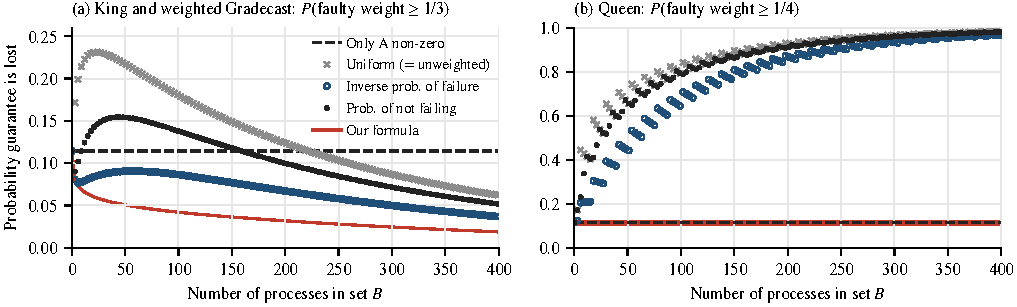
\includegraphics[width=\textwidth]{figures/failure_probability.pdf}
\caption{Probability that the faulty weight reaches the algorithm's bound, versus $|B|$ ($|A|=6$, $f_A=0.1$, $f_B=0.3$; exact). (a) recreates Garg and Bridgman's Fig.~4 and applies to both weighted King and WGC. (b) is the same for weighted Queen's bound of $1/4$. The red line is our weight formula from Section~\ref{sec:eval}; at $1/4$ it gives $B$ weight 0, which is the only-A line.}\label{fig:fail}
\end{figure*}

\section{Implementation}\label{sec:impl}

The code is a Python package of about 2{,}400 lines (\texttt{byzantine/}), plus unit tests and an experiment script (\texttt{run\_experiments.py}). \texttt{network.py} runs the processes in lock-step: each honest process is a Python generator that hands over one step's outgoing messages and gets back that step's incoming ones, and the simulator counts the bits honest processes send. Weights are scaled to integers and $\rho$ is a fraction, so every threshold check is exact. In WGC, all $p$ gradecasts of an iteration run in parallel, and each echo or support message is one vector with an entry per leader; a test checks this against a simple loop-based version.

\emph{Adversary.} One adversary controls all the faulty processes. It is \emph{rushing}: in each step it sees every honest message before it picks what the faulty processes send. The strategies are \emph{silent} (crash at the start), \emph{crash}, \emph{random} messages, \emph{flip}, \emph{equivocate}, and the two attacks we use most:
\begin{itemize}
\item \emph{Split vote.} Each step, the adversary splits the honest processes into two camps by the value they just sent. Faulty processes push each camp toward its own value, and a faulty coordinator tells the camps opposite values.
\item \emph{Stagger} (against WGC). Each iteration it uses up one faulty leader, getting it grade 1 from some honest processes and 0 from the rest, and sets up the other faulty leaders so this one tips the majority. The two groups then end the iteration with different values. The groups are picked greedily, so it is a strong attack but not a proven worst case.
\end{itemize}

\emph{Testing.} Unit tests check agreement, validity and termination for every algorithm, every $N\le16$ and every tolerated $t$, against every adversary, several input patterns and fault placements, and on random weighted systems with zero weights. A model checker that tries every Byzantine behavior shows that Queen ($N=5,t=1$) and King ($N=4,t=1$) are safe and finds counterexamples one step past each bound; it does not cover WGC. All 16 tests pass, and a fresh sweep of 26{,}208 runs of all three algorithms ($N$ from 4 to 49, every $t$ up to the bound, 7 adversaries) found no violations.

\section{Evaluation}\label{sec:eval}

\subsection{Setup}
We use the same setup as Garg and Bridgman's Figs.~4 and~5~\cite{garg2011}. Group $A$ has 6 processes that each fail with probability $f_A=0.1$, and group $B$ has 0 to 399 processes that each fail with probability $f_B=0.3$, all independently. Like the original, we only plot sizes where $|A|+|B|$ is divisible by 3. Each weighting gives every process in a group the same weight:
\begin{itemize}
\item \emph{only A non-zero}: $B$ gets weight 0;
\item \emph{uniform}: the unweighted algorithms;
\item \emph{inverse probability of failure}: $w_A:w_B=3:1$;
\item \emph{probability of not failing}: $w_A:w_B=9:7$.
\end{itemize}
King and WGC use $\rho=1/3-10^{-6}$.\footnote{The algorithms need $\rho<1/3$. With these integer weights, any faulty fraction below $1/3$ is at least $10^{-4}$ below it, so this $\rho$ gives the same results.}

From the failure model we compute three things exactly: (1) the chance that the faulty weight reaches the algorithm's limit ($1/3$ for King and WGC, $1/4$ for Queen; hitting it exactly counts as failing); (2) $\alpha_\rho$ and $\capr$; and (3) WGC's expected bound $E[\min(F+3,\capr)]$ over runs that stay within the limit, where $F$ is the number of failed positive-weight processes. We also simulate WGC: for each weighting and $|B|\in\{0,6,12,18,30,42,60,90,120\}$ we draw 20 failure sets within the limit and run each one against the stagger attack and against silent faults (1{,}440 runs).

\subsection{Chance the guarantee is lost}

Fig.~\ref{fig:fail}(a) recreates Garg and Bridgman's Fig.~4. King and WGC tolerate the same faulty weight, so they lose their guarantee in exactly the same runs and share one curve per weighting. Uniform weights are worst for small $|B|$, peaking at 0.231 at $|B|=24$. Inverse-failure weights are the safest of the weightings that give $B$ any weight: they never go above 0.114, and at $|B|=399$ they give 0.037, against 0.052 (probability of not failing), 0.062 (uniform) and 0.114 (only A). Only-A stays flat at $P(\ge 2\text{ of the 6 fail})=0.114$, since two failures already reach exactly $1/3$. Fig.~\ref{fig:fail}(b) shows why Queen is a bad fit here. Since $f_B=0.3>1/4$, $B$'s faulty weight is expected to be over Queen's bound already, and every weighting that gives $B$ any weight loses the guarantee in over 96\% of runs at $|B|=399$.

\begin{figure*}[t]
\centering
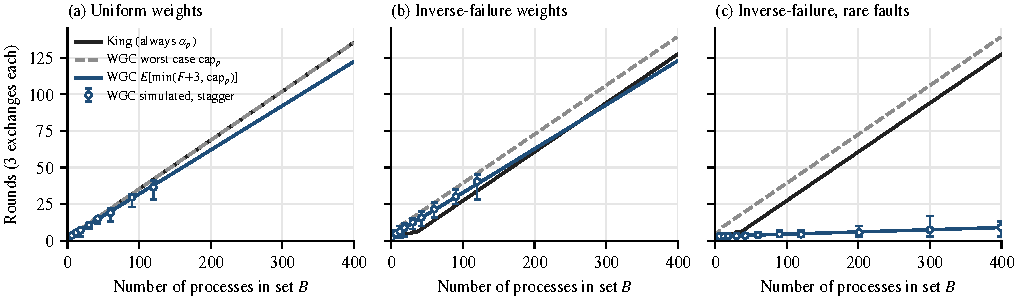
\includegraphics[width=\textwidth]{figures/king_vs_gradecast.pdf}
\caption{Rounds to decide (one round = three message exchanges for both algorithms), versus $|B|$, safe runs only. Lines are exact: King's $\alpha_\rho$, WGC's worst case $\capr$, and WGC's bound $\min(F+3,\capr)$ averaged over the failure model. Circles are simulated WGC runs against the stagger attack (mean, with bars from minimum to maximum, over 20 failure draws). (a) and (b) use Garg and Bridgman's failure rates; (c) uses the rare rates of Section~\ref{sec:update}.}\label{fig:kvg}
\end{figure*}

\emph{Choosing weights.} These four weightings are rules of thumb, and a simple formula does better. Say process $i$ fails with probability $p_i$ and the bound is $\tau$. If we treat the faulty weight as roughly normal, the guarantee is safest when the margin $\sum_i w_i(\tau-p_i)$ is as large as possible compared with its standard deviation $\sqrt{\sum_i w_i^2p_i(1-p_i)}$, and that happens when \[ w_i \propto \max\Bigl(0,\ \frac{\tau-p_i}{p_i(1-p_i)}\Bigr). \] So any process that fails at least as often as the bound gets weight 0. For $\tau=1/3$ this gives $w_A:w_B\approx16.3:1$, much more lopsided than inverse-failure's $3:1$. Fig.~\ref{fig:fail}(a) shows it in red: it is at or below every other weighting for every $|B|$, and at $|B|=399$ it loses the guarantee with probability 0.019, about half of inverse-failure's 0.037. An exact search over every ratio $w_A:w_B$ gets down to 0.016, and up to $|B|=60$ the formula matches it to four decimals. For Queen's $\tau=1/4$, the formula gives $B$ weight 0, which is the only-A weighting, also the best of the four in Fig.~\ref{fig:fail}(b).

From here on we compare King and WGC.

\subsection{Rounds needed by weighted King}
Fig.~\ref{fig:king} recreates Garg and Bridgman's Fig.~5. Uniform weights give the unweighted $f+1$ with $f=\lfloor (N-1)/3\rfloor$, which is 135 rounds at $|B|=399$ ($N=405$). Inverse-failure weights need 127, and probability-of-not-failing weights need 134. Only-A needs just 2 rounds for every $|B|$, but pays for it with the constant 11.4\% risk from Fig.~\ref{fig:fail}. Our formula needs at most 8 rounds up to $|B|=201$ and 74 at $|B|=399$, because its six heavy A processes cover most of $\rho$ on their own.

\subsection{Weighted King versus weighted Gradecast}
\emph{Uniform weights} (Fig.~\ref{fig:kvg}(a)). Here $\capr=\alpha_\rho=t+1$, so WGC's worst case is the same as King's. Early stopping brings the expected round bound down to 122.0 at $|B|=399$, against King's 135, about 10\% less. The saving is small because about 30\% of $B$ actually fails, so $F$ ends up close to $t$.

\emph{Inverse-failure weights} (Fig.~\ref{fig:kvg}(b)). Here the heaviest-versus-lightest difference shows up. The 6 heavy A processes bring King's $\alpha_\rho$ down (14 at $|B|=60$, 127 at $|B|=399$). WGC's worst case depends on how many light B processes fit under $\rho$, which is more: 26 and 139. WGC's expected bound stays above King's $\alpha_\rho$ up to $|B|=258$ and only drops below it from $|B|=261$. With not-failing weights, $\capr>\alpha_\rho$ for every $|B|\ge 3$.

\emph{Formula weights.} These favor King even more. Its $\alpha_\rho$ drops to 74 at $|B|=399$, while WGC's expected bound stays at 123.1 and its worst case $\capr$ rises to 166. King is at or below WGC's expected bound at every $|B|$, so the safest weighting is also the one that suits King best.

\emph{Simulation.} All 1{,}440 simulated WGC runs reached agreement and validity. None took longer than its own bound $\min(F+3,\capr)$, and the stagger attack hit that bound exactly in 702 of 720 runs. In 321 of those (78 with uniform weights) it reached $F+3<\capr$, so the $F+3$ bound is tight. The simulated averages follow the expected-bound curve, but not always below it: for inverse weights at $|B|=120$ the average is 40.5 against an expected 38.8, because the 20 sampled failure sets had more faults than average. Against processes that are silent, WGC finished within 3 rounds in every run.

\emph{Rare faults.} King's rounds depend only on the weights, and WGC's mostly on how many processes fail, which with Garg and Bridgman's rates is about 120 at $|B|=399$. Fig.~\ref{fig:kvg}(c) uses the per-instance rates of Section~\ref{sec:update} instead: A fails with probability 0.005 and B with 0.015. King still needs 127 rounds at $|B|=399$, while WGC's expected bound is 9.0 for every weighting that gives B weight; 240 simulated stagger runs up to $|B|=399$ all reached agreement, stayed within their bound, and averaged 9.1 rounds at $|B|=399$. King can catch up by moving weight onto A: at $60:1$ it needs 5 rounds and loses the guarantee with probability about $10^{-10}$. So WGC wins when faults are rare and there is no small reliable group to put the weight on.

\begin{figure*}[t]
\centering
\begin{minipage}[t]{\columnwidth}\vspace{0pt}\centering
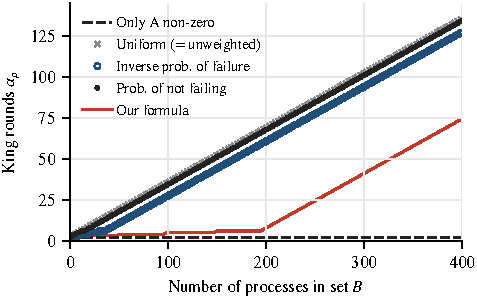
\includegraphics[width=\linewidth]{figures/king_rounds.pdf}
\end{minipage}\hfill
\begin{minipage}[t]{\columnwidth}\vspace{0pt}\centering
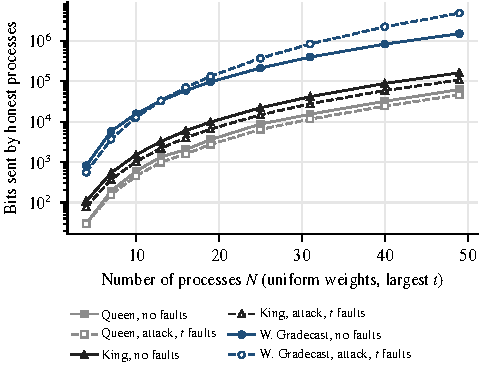
\includegraphics[width=\linewidth]{figures/messages.pdf}
\end{minipage}

\begin{minipage}[t]{\columnwidth}
\caption{Rounds $\alpha_\rho$ that weighted King always runs, versus $|B|$ (recreates Garg and Bridgman's Fig.~5), plus our weight formula in red.}\label{fig:king}
\end{minipage}\hfill
\begin{minipage}[t]{\columnwidth}
\caption{Bits sent by honest processes in one agreement instance, uniform weights, largest tolerated $t$, inputs alternating 0/1. ``Attack'' means $t$ faulty processes running split vote (Queen, King) or stagger (WGC). Log scale.}\label{fig:msgs}
\end{minipage}
\end{figure*}

\begin{figure*}[b]
\centering
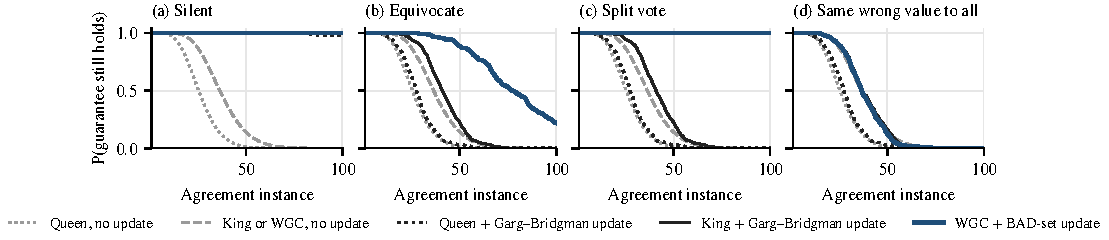
\includegraphics[width=\textwidth]{figures/weight_update.pdf}
\caption{Weight updates when processes fail over time: the share of runs whose faulty weight is still below the bound at each agreement instance (6 A and 30 B processes, weights $3:1$, 200 runs per line). Gray lines are exact and use no update. In (a), all three update schemes stay near 1.}\label{fig:update}
\end{figure*}

\subsection{Message complexity}
Fig.~\ref{fig:msgs} measures one run with uniform weights for $N$ from 4 to 49. We count bits rather than messages, because the simulator packs all $p$ gradecasts' echoes into one vector message, which would make WGC's message count look small. Queen and King send the same amount no matter what the adversary does; the only difference is that faulty processes do not count as honest senders. At $N=49$ ($t=16$), King sends 161{,}568 bits over 17 rounds. With no faults, WGC decides in 3 iterations (9 steps instead of King's 51) but sends 1{,}509{,}984 bits, $9.3\times$ as many. Under the stagger attack it runs all $t+1=17$ iterations and sends 4{,}873{,}248 bits, $45\times$ King's 107{,}808. One WGC iteration costs about as much as $p$ King rounds, so early stopping saves time but not bandwidth. Weights only change how many rounds run (zero-weight processes send nothing), so for any weighting the cost is the per-round cost depends on p; weights change it through p and through the round counts in Figs.~\ref{fig:kvg} and~\ref{fig:king}.

\subsection{Updating weights over time}\label{sec:update}
So far the weights never change. Garg and Bridgman also describe updating them between agreement instances: a process caught misbehaving gets weight 0. We tested this with 6 A and 30 B processes (weights $3:1$) over 100 agreement instances in a row, where before each instance every A process fails with probability 0.005 and every B process with probability 0.015, and stays faulty. Without updates, the guarantee is lost by instance 26 for Queen and 37 for King and WGC (medians).

Queen and King use Garg and Bridgman's rule, which flags processes that send nothing or garbage and coordinators that contradict a clear majority (we apply the Queen rule to King too); WGC also flags everyone in its $\BAD$ sets. Rather than simulate the agreements that decide whom to drop, we assume the worst outcome validity allows, so an honest process is never dropped. All 143{,}252 simulated instances (200 runs per line) reached agreement and validity.

Fig.~\ref{fig:update} shows the results. Silent processes are easy: every scheme drops them, and the guarantee lasts all 100 instances in 98--100\% of runs. Against processes that actively lie, Garg and Bridgman's rule catches almost nothing (under one process per run on average), so Queen and King lose the guarantee about when they would with no update (instance 28 instead of 26 for Queen, 41 instead of 37 for King). WGC's $\BAD$ sets do much better. Against split vote they caught nearly every faulty process, and the guarantee lasted all 100 instances in every run. Against equivocators they dropped 13.4 faulty processes per run on average, which pushed the median loss from instance 37 to 69.5, and 22\% of runs lasted all 100. Processes that tell everyone the same wrong value are invisible to every scheme, since they look like honest processes with a different input, so WGC loses the guarantee at instance 37, as with no update.

\section{Discussion and Limitations}\label{sec:disc}

\emph{Limitations.} (i) The stagger attack is a heuristic. A stronger adversary might push WGC to $\min(F+3,\capr)$ more often, but by Proposition~\ref{prop:wgc} never past it. That is also why the curves in Fig.~\ref{fig:kvg} are bounds, not measured averages. (ii) The simulator assumes synchronous rounds and reliable channels; it does not model real network delays or asynchrony. (iii) Bits are counted with a simple model (2 bits per value, plus 8 bits of framing per vector). (iv) Like Garg and Bridgman, we assume processes fail independently. (v) The weight-update test assumes the worst outcome of the agreements that decide whom to drop, rather than simulating them.

\section{Conclusion}\label{sec:concl}

We built a weighted Gradecast consensus by swapping count thresholds for weight thresholds, and argued that it is correct for $\rho<1/3$, like weighted King, and stops within $\min(F+3,\capr)$ iterations. On Garg and Bridgman's two-group setup, weights let many light processes fail safely; inverse-failure weights are the safest of the four weightings, and our formula roughly halves their risk. WGC finishes in 2--3 iterations when faulty processes are silent from the start, and its blacklists make a much better weight-update rule than Garg and Bridgman's, except against processes that lie consistently. It pays with far more traffic and, with uneven weights, a worst case set by the lightest processes. So WGC fits best when Byzantine faults are rare, there is no small reliable group for King to lean on, and latency matters more than bandwidth.
\bibliographystyle{IEEEtran}
\bibliography{references}

\section{AI Disclosure}
AI was used to challenge the ideas presented, format the paper, and review bugs.

\end{document}